\documentclass{article}
\usepackage{graphicx}
\graphicspath{{./images/}}
\usepackage[a4paper, margin=2cm]{geometry}
\usepackage[]{enumitem}
\usepackage{float}
\usepackage[]{titling}
\usepackage{hyperref}

\setlength{\droptitle}{-5em}

\title{Assignment 1 Report}
\author{Liam Watson}
\date{\today}

\begin{document}
	
	\maketitle
	
	\section{Introduction}
	This report details answers to key questions posed throughout the Digital Watch Part 1 Assignment and analyses all waveforms given by each module using a Testbench. We aim to highlight key findings and confirm all output behaves as expected after testing.\\
	\\
	\noindent Repository fpga-digital-watch forked and seven\_segment module completed locally. Changes committed and pushed as backup to GitHub. 
	
	\section{Report 1}
	\begin{figure}[H]
		\centering
		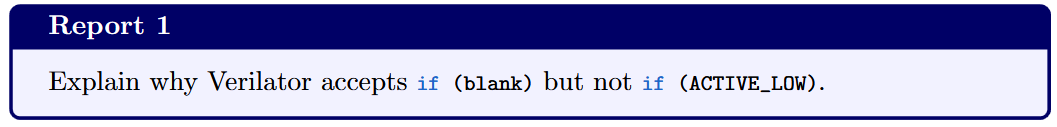
\includegraphics[width=\linewidth]{q_report1}
		\caption{Screenshot taken from Digital\_Watch\_Part\_1.pdf}
	\end{figure}
	
	Verilator only accepts \textbf{blank} otherwise the signal \textbf{blank} is not used in the instance seven\_segment.
	
	\section{Report 2}
	\begin{figure}[H]
		\centering
		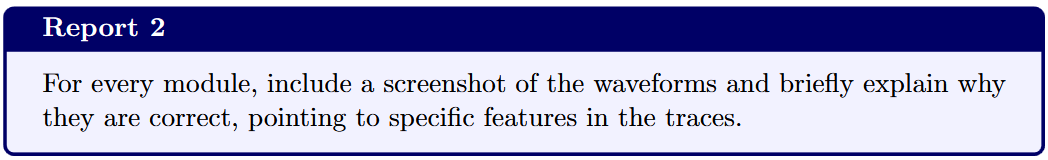
\includegraphics[width=\linewidth]{q_report2}
		\caption{Screenshot taken from Digital\_Watch\_Part\_1.pdf}
	\end{figure}
	
	\subsection{Seven Segment Display}
	
	\begin{figure}[H]
		\centering
		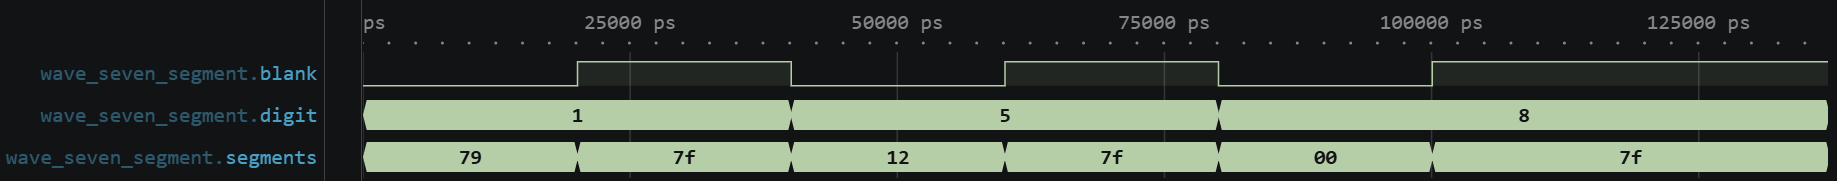
\includegraphics[width=\linewidth, height=0.1\textheight]{seven_segment_waveform}
		\caption{Measured waveform for seven\_segment.sv}
	\end{figure}
	
	The waveform for seven\_segment displays inputs \textbf{blank}, \textbf{digit}, and output \textbf{segments}. We observe that:
	
	\begin{itemize}[noitemsep]
		\item When \textbf{blank} is low \textbf{segments} corresponds to the appropriate display output (e.g. when \textbf{digit} = 1, \textbf{segments} = 79 or 7'b1111001). 
		\item When \textbf{blank} is high \textbf{segments} is set to 7F or 7'b1111111 which turns off all segments.
	\end{itemize}
	
	\subsection{Parameterised Up-Down Counter with Enable}
	
	\begin{figure}[H]
		\centering
		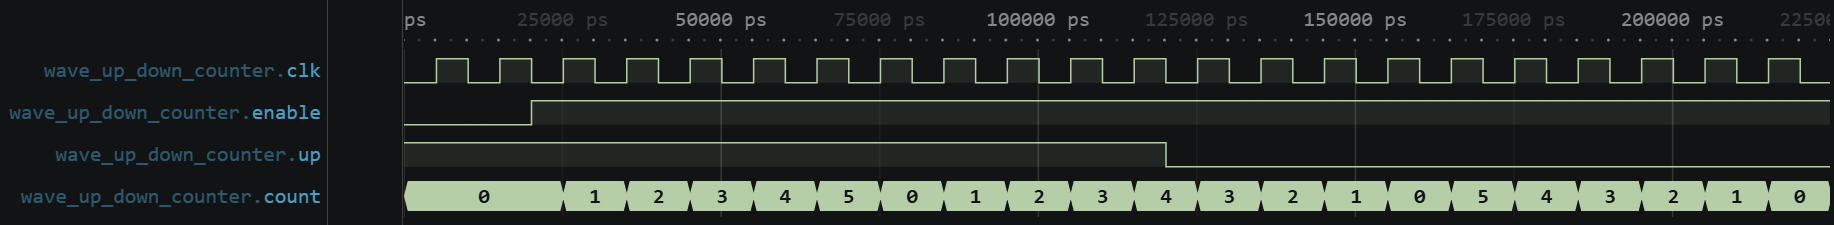
\includegraphics[width=\linewidth, height=0.1\textheight]{up_down_counter_waveform}
		\caption{Measured waveform for up\_down\_counter.sv}
	\end{figure}
	
	The waveform displays inputs \textbf{clk}, \textbf{enable}, \textbf{up} and output \textbf{count}. \textbf{MAX} is set to 5 and \textbf{WIDTH} set to 3 in our Testbench. We observe that:
	
	\begin{itemize}[noitemsep]
		\item When \textbf{enable} is low \textbf{count} holds its current value at 0. 
		\item When \textbf{enable} and \textbf{up} are high \textbf{count} increments and wraps after \textbf{count} = 5. 
		\item  When \textbf{enable} is high and \textbf{up} is low \textbf{count} decrements and wraps after \textbf{count} = 0. 
	\end{itemize}
	
	\subsection{Binary to Binary-Coded Decimal}
	
	\begin{figure}[H]
		\centering
		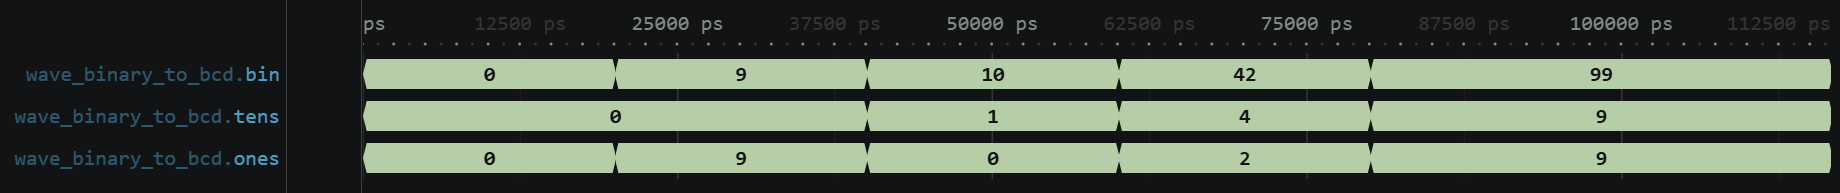
\includegraphics[width=\linewidth, height=0.1\textheight]{binary_to_bcd_waveform}
		\caption{Measured waveform for binary\_to\_bcd.sv}
	\end{figure}
	
	The waveform displays inputs \textbf{bin}, and outputs \textbf{tens}, and \textbf{ones}. We observe that:
	
	\begin{itemize}[noitemsep]
		\item \textbf{bin} displays input digit.
		\item \textbf{tens} corresponds with 10s column of \textbf{bin}.
		\item \textbf{ones} corresponds with 1s column of \textbf{bin}.
	\end{itemize}
	
	\subsection{Cascaded Hour-Minute-Second Counter with Enable}
	
	\begin{figure}[H]
		\centering
		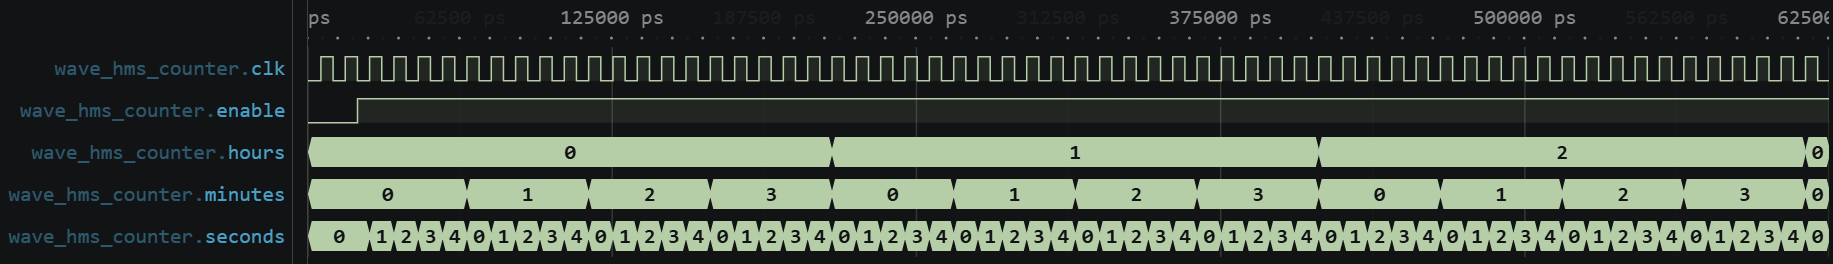
\includegraphics[width=\linewidth, height=0.1\textheight]{hms_counter_waveform}
		\caption{Measured waveform for hms\_counter.sv}
	\end{figure}
	
	The waveform displays inputs \textbf{clock}, \textbf{enable} and outputs \textbf{hours}, \textbf{minutes} and \textbf{seconds}. We observe that:
	
	\begin{itemize}[noitemsep]
		\item When \textbf{enable} is low all outputs hold current value.
		\item When \textbf{enable} is high \textbf{seconds} increments every rising clock edge.
		\item \textbf{minutes} increments after \textbf{seconds} reaches its max value.
		\item \textbf{hours} increments after \textbf{minutes} reaches its max value.
		\item each counter wraps after its max value is reached.
	\end{itemize}
	
		\begin{itemize}[noitemsep]
		\item \textbf{bin} displays input digit.
		\item \textbf{tens} corresponds with 10s column of \textbf{bin}.
		\item \textbf{ones} corresponds with 1s column of \textbf{bin}.
	\end{itemize}
	
	\subsection{Modulo N Counter}
	
	\begin{figure}[H]
		\centering
		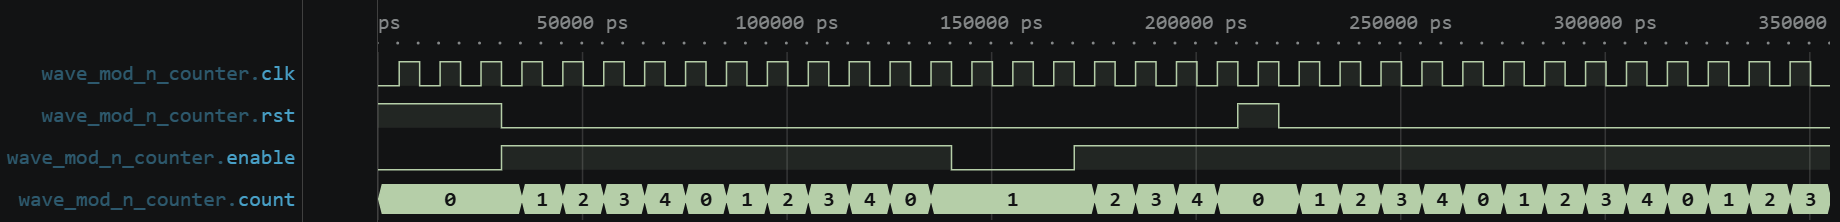
\includegraphics[width=\linewidth, height=0.1\textheight]{mod_n_counter_waveform}
		\caption{Measured waveform for mod\_n\_counter.sv}
	\end{figure}
	
	The waveform displays inputs \textbf{clk}, \textbf{rst}, and \textbf{enable} and output \textbf{count}. We observe that:
	
	\begin{itemize}[noitemsep]
		\item When \textbf{enable} is low all outputs hold current value.
		\item When \textbf{rst} is high \textbf{count} is reset to 0 and has priority over \textbf{enable}.
		\item When \textbf{enable} is high and \textbf{rst} is low \textbf{count} increments every rising clock edge.
		\item \textbf{count} wraps after \textbf{N - 1} is reached.
	\end{itemize}
	
	\subsection{Restartable Rate Generator}
	
		\begin{figure}[H]
		\centering
		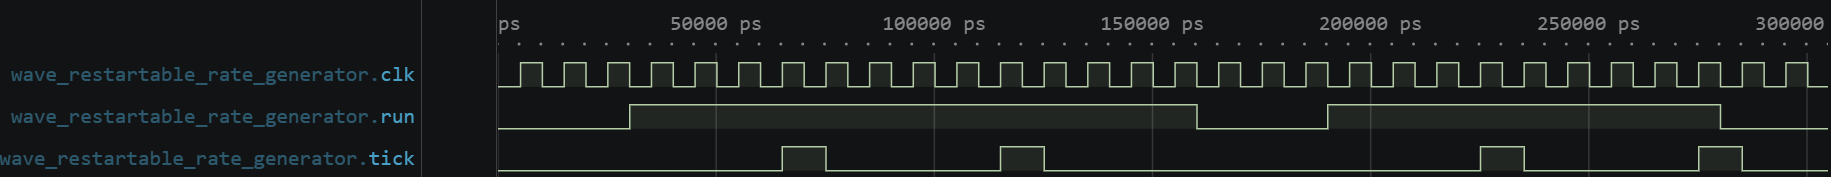
\includegraphics[width=\linewidth, height=0.1\textheight]{restartable_rate_generator_waveform}
		\caption{Measured waveform for restartable\_rate\_generator.sv}
	\end{figure}
	
	The waveform displays inputs \textbf{clk}, and \textbf{run}, and output \textbf{tick}. We observe that:
	
	\begin{itemize}[noitemsep]
		\item When \textbf{run} is low \textbf{tick} is low.
		\item When \textbf{run} is high for \textbf{CYCLE\_COUNT - 1} rising edges \textbf{tick} outputs a one cycle pulse.
	\end{itemize}
	
	\subsection{Top Time Display V1}
	
	\begin{figure}[H]
		\centering
		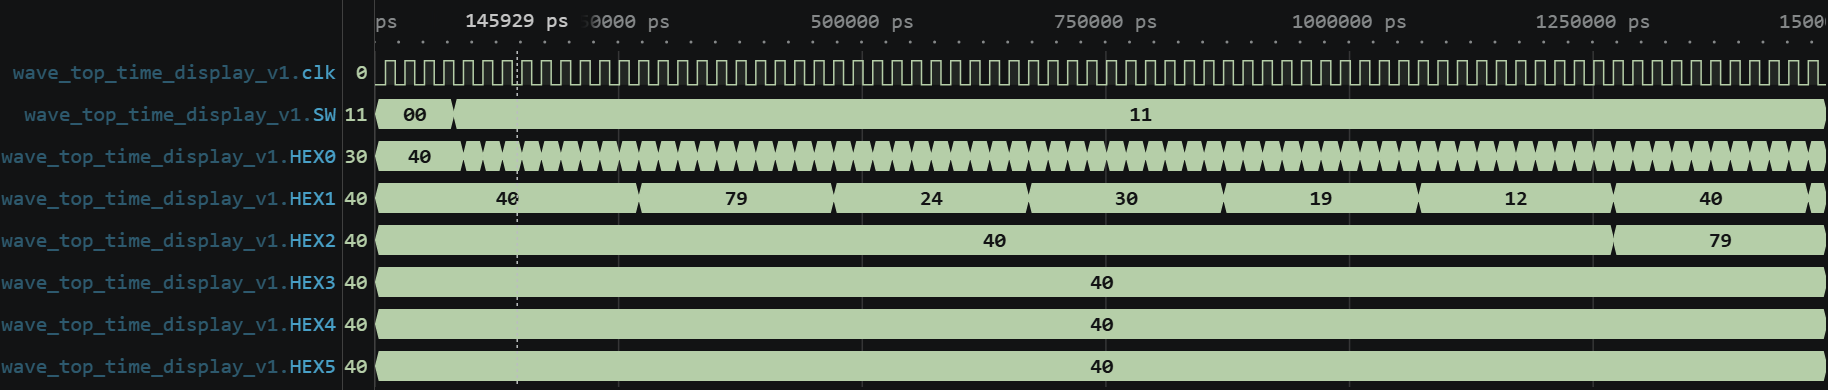
\includegraphics[width=\linewidth, height=0.1\textheight]{top_time_display_v1_waveform}
		\caption{Measured waveform for top\_time\_display\_v1.sv}
	\end{figure}
	
	The waveform displays inputs \textbf{clk}, and \textbf{SW}, and outputs \textbf{HEX0}, \textbf{HEX1}, \textbf{HEX2}, \textbf{HEX3}, \textbf{HEX4}, and \textbf{HEX5}. We observe that:
	
	\begin{itemize}[noitemsep]
		\item When \textbf{SW} is 00 counter holds 00:00:00.
		\item When \textbf{SW} is high second counter increments every cycle and minutes increments to 1 when seconds rolls over from 59 to 0.
	\end{itemize}
	
	\subsection{Pulse Width Generator}
	
	\begin{figure}[H]
		\centering
		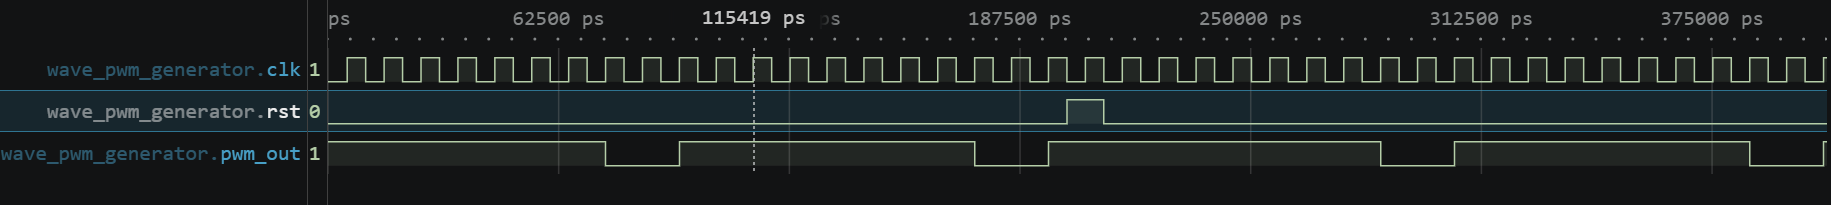
\includegraphics[width=\linewidth, height=0.1\textheight]{pwm_generator_waveform}
		\caption{Measured waveform for pwm\_generator.sv}
	\end{figure}
	
	The waveform displays inputs \textbf{clk}, and \textbf{rst}, and output \textbf{pwm\_out}. We observe that:
	
	\begin{itemize}[noitemsep]
		\item When \textbf{pwm\_out} has period of \textbf{PERIOD\_CYCLES} and is high for first [DUTY\_CYLES].
		\item When \textbf{rst} is high \textbf{pwm\_out} stays high next clock edge.
	\end{itemize}
	
	\subsection{Rising Edge Detector}
	
	\begin{figure}[H]
		\centering
		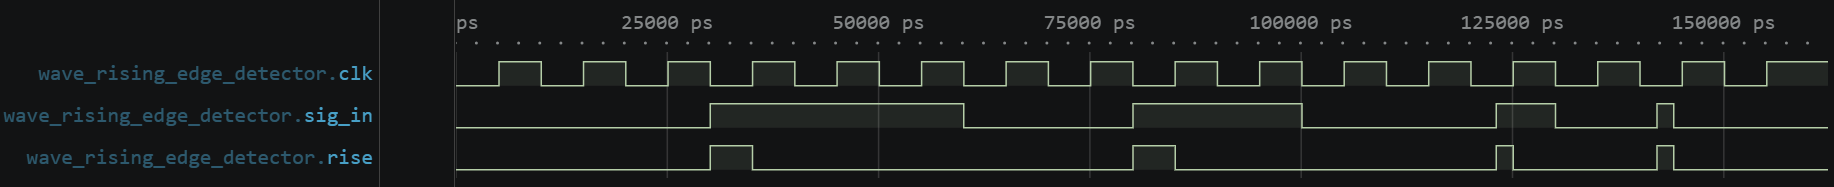
\includegraphics[width=\linewidth, height=0.1\textheight]{rising_edge_detector_waveform}
		\caption{Measured waveform for rising\_edge\_detector.sv}
	\end{figure}
	
	The waveform displays inputs \textbf{clk}, and outputs \textbf{sig\_in} and \textbf{rise}. We observe that:
	
	\begin{itemize}[noitemsep]
		\item When \textbf{sig\_in} is high \textbf{rise} is high for remainder of clock cycle.
	\end{itemize}
	
	\subsection{Button Hold Detect}
	
	\begin{figure}[H]
		\centering
		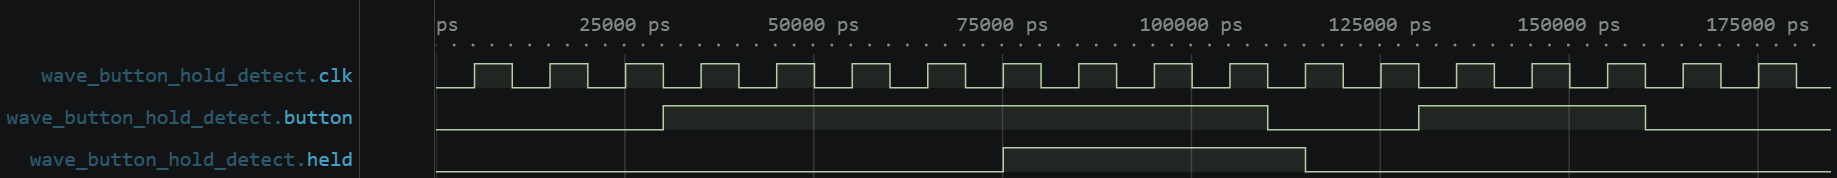
\includegraphics[width=\linewidth, height=0.1\textheight]{button_hold_detect_waveform}
		\caption{Measured waveform for button\_hold\_detect.sv}
	\end{figure}
	
	The waveform displays inputs \textbf{clk} and \textbf{button} and output \textbf{held}. We observe that:
	
	\begin{itemize}[noitemsep]
		\item \textbf{held} goes high after \textbf{button} is pressed for \textbf{HOLD\_CYCLES} only.
		\item \textbf{held} goes low after button has been released.
	\end{itemize}
	
	\subsection{Button Hold Pulse}
	
	\begin{figure}[H]
		\centering
		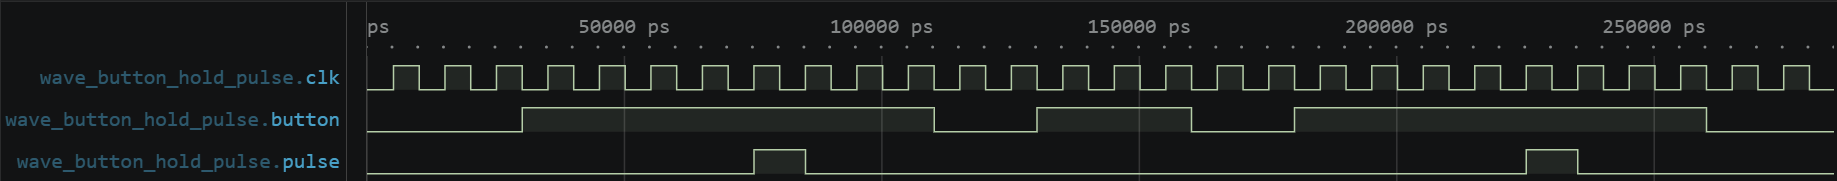
\includegraphics[width=\linewidth, height=0.1\textheight]{button_hold_pulse_waveform}
		\caption{Measured waveform for button\_hold\_pulse.sv}
	\end{figure}
	
	The waveform displays inputs \textbf{clk} and \textbf{button} and output \textbf{pulse}. We observe that:
	
	\begin{itemize}[noitemsep]
		\item \textbf{pulse} goes high for a single clock cycle after \textbf{button} is pressed for appropriate \textbf{HOLD\_CYCLES} within \textbf{button\_hold\_detect} module.
	\end{itemize}
	
	\subsection{Button Auto Repeat}
	
	\begin{figure}[H]
		\centering
		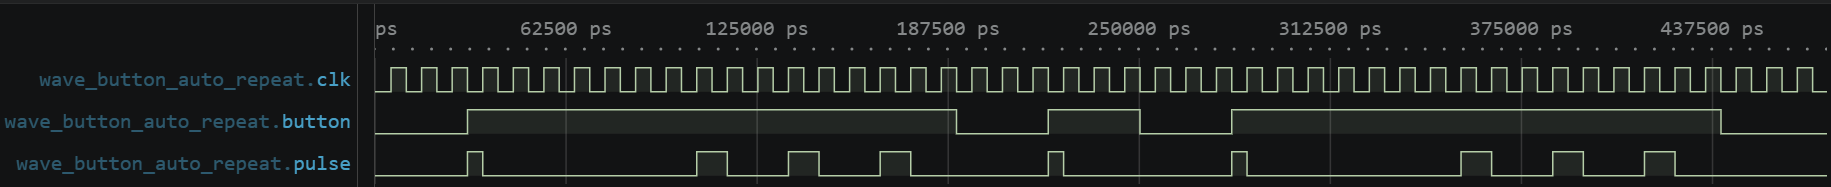
\includegraphics[width=\linewidth, height=0.1\textheight]{button_auto_repeat_waveform}
		\caption{Measured waveform for button\_auto\_repeat.sv}
	\end{figure}
	
	The waveform displays inputs \textbf{clk} and \textbf{button} and output \textbf{pulse}. We observe that:
	
	\begin{itemize}[noitemsep]
		\item \textbf{pulse} goes high for a single clock cycle after \textbf{button} is pressed.
		\item \textbf{pulse} train after \textbf{button} has been held for \textbf{HOLD\_CYCLES - REPEAT\_CYCLES + 1}.
	\end{itemize}
	
	\subsection{Arming Latch}
	
	\begin{figure}[H]
		\centering
		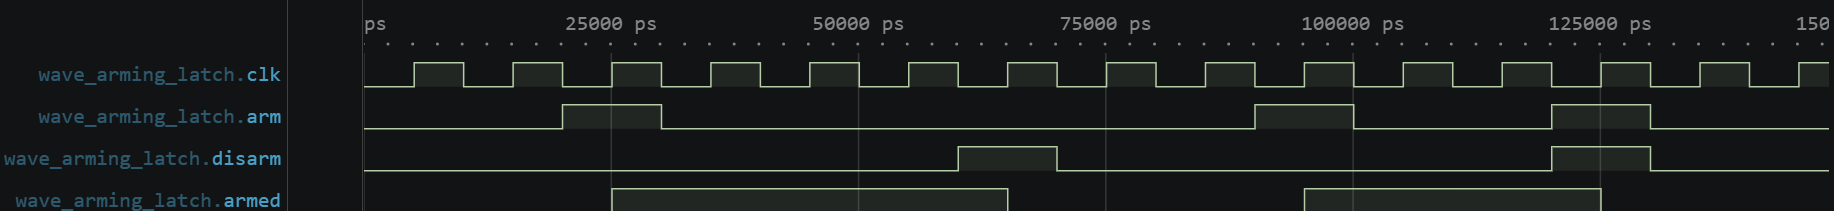
\includegraphics[width=\linewidth, height=0.1\textheight]{arming_latch_waveform}
		\caption{Measured waveform for arming\_latch.sv}
	\end{figure}
	
	The waveform displays inputs \textbf{clk}, \textbf{arm}, and \textbf{disarm} and output \textbf{armed}. We observe that:
	
	\begin{itemize}[noitemsep]
		\item \textbf{armed} goes low next rising edge if \textbf{disarm} is high.
		\item \textbf{armed} goes high if \textbf{arm} is high and \textbf{disarm} is low.
	\end{itemize}
	
	\subsection{Edit Mode Select}
	
	\begin{figure}[H]
		\centering
		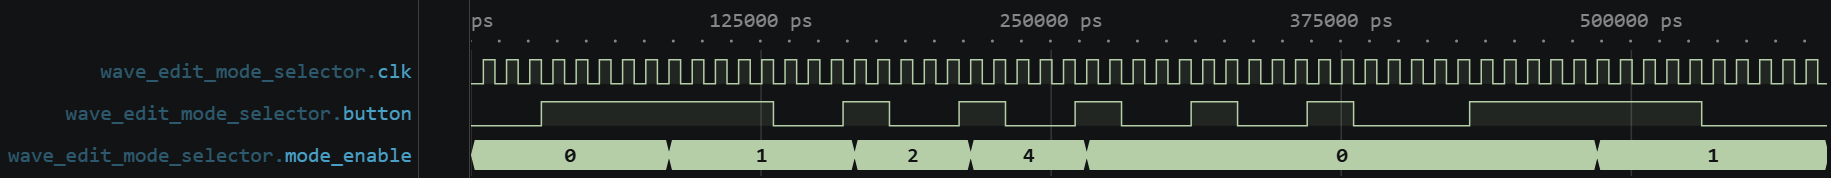
\includegraphics[width=\linewidth, height=0.1\textheight]{edit_mode_select_waveform}
		\caption{Measured waveform for edit\_mode\_select.sv}
	\end{figure}
	
	The waveform displays inputs \textbf{clk}, \textbf{buton}, and output \textbf{mode\_enable}. We observe that:
	
	\begin{itemize}[noitemsep]
		\item \textbf{mode\_enable} increments if \textbf{button} is held high for \textbf{long\_press}.
		\item \textbf{mode\_enable} then increments to next mode after \textbf{press}
		\item Once \textbf{mode\_enable} passes last mode must hold for \textbf{long\_press} again to enter mode select.
	\end{itemize}
	
	\subsection{Editable Counter}
	
	\begin{figure}[H]
		\centering
		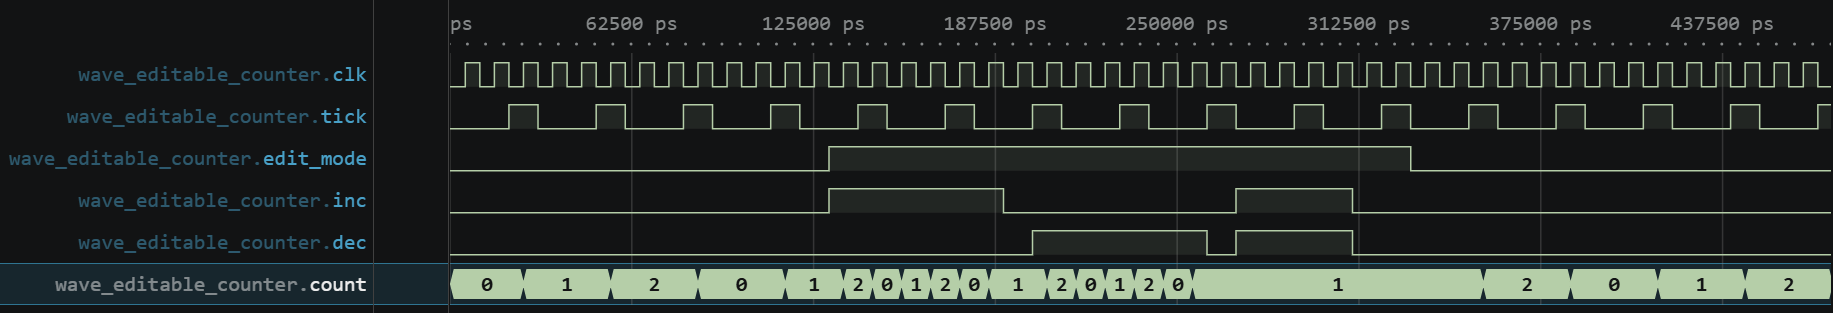
\includegraphics[width=\linewidth, height=0.1\textheight]{editable_counter_waveform}
		\caption{Measured waveform for editable\_counter.sv}
	\end{figure}
	
	The waveform displays inputs \textbf{clk}, \textbf{tick}, \textbf{edit\_mode}, \textbf{inc}, \textbf{dec} and output \textbf{count}. We observe that:
	
	\begin{itemize}[noitemsep]
		\item When \textbf{edit\_mode} is low \textbf{count} increments every tick.
		\item When \textbf{edit\_mode} is and \textbf{inc} high \textbf{count} increments.
		\item When \textbf{edit\_mode} is high and \textbf{dec} is high \textbf{count} decrements.
		\item When both \textbf{inc} and \textbf{inc} are high when \textbf{edit\_mode} is high\textbf{count} holds value.
	\end{itemize}
	
	\subsection{Key Synchroniser}
	
	\begin{figure}[H]
		\centering
		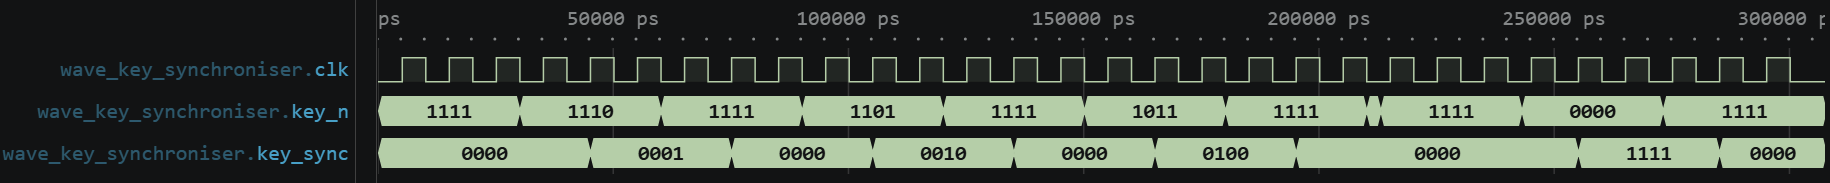
\includegraphics[width=\linewidth, height=0.1\textheight]{key_synchroniser_waveform}
		\caption{Measured waveform for key\_synchroniser.sv}
	\end{figure}
	
	The waveform displays inputs \textbf{clk}, \textbf{key\_n}, and output \textbf{key\_sync}. We observe that:
	
	\begin{itemize}[noitemsep]
		\item \textbf{key\_sync} displays a one cycle delayed inverted output of \textbf{key\_n}.
	\end{itemize}
	
	\subsection{Decimal Display Driver}
	
	\begin{figure}[H]
		\centering
		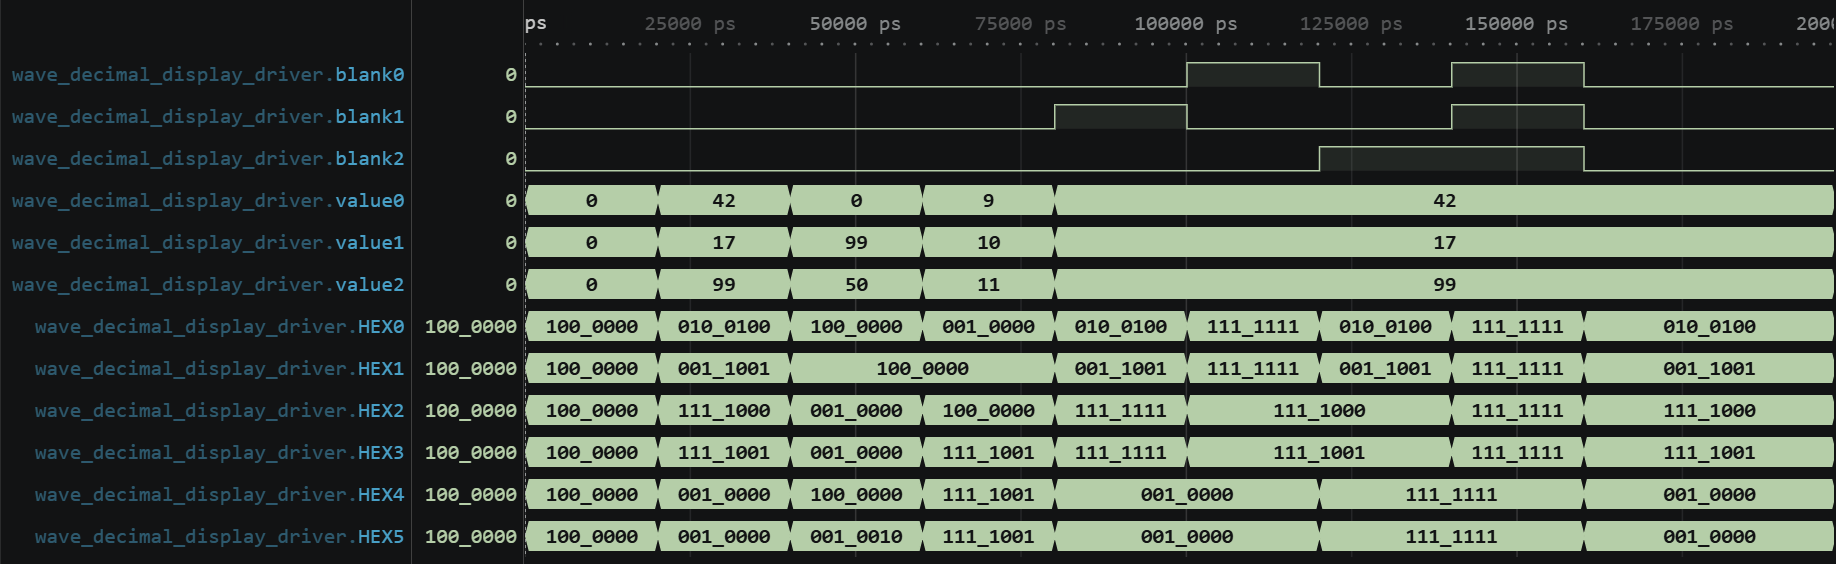
\includegraphics[width=\linewidth, height=0.2\textheight]{decimal_display_driver_waveform}
		\caption{Measured waveform for decimal\_display\_driver.sv}
	\end{figure}
	
	The waveform displays inputs \textbf{blank[n]}, \textbf{value[n]}, and outputs \textbf{HEX0 - HEX5}. We observe that:
	
	\begin{itemize}[noitemsep]
		\item \textbf{value} is converted to the corresponding tens and ones values and displayed on our \textbf{HEX} outputs.
		\item  When \textbf{blank} is asserted the corresponding \textbf{HEX} displays are turned off indicated by the output \textbf{111\_1111}.
	\end{itemize}
	
	\subsection{User Top Watch V1}
	
	\begin{figure}[H]
		\centering
		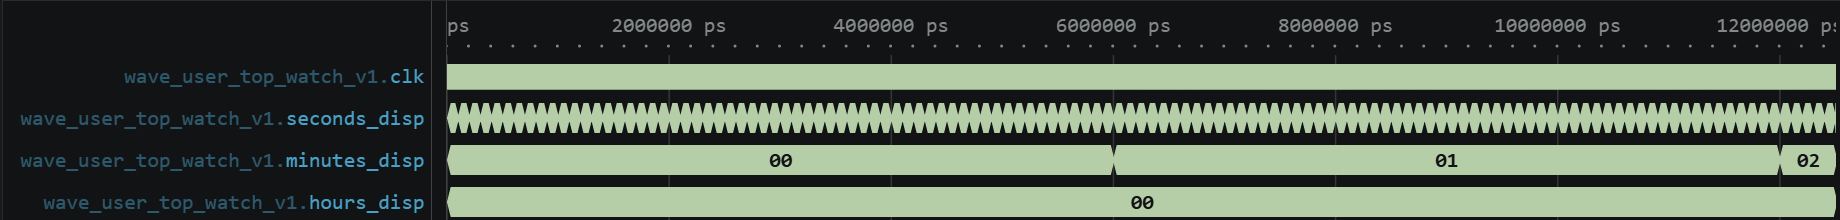
\includegraphics[width=\linewidth, height=0.1\textheight]{user_top_watch_v1_waveform}
		\caption{Measured waveform for user\_top\_watch\_v1.sv}
	\end{figure}
	
	The waveform displays inputs \textbf{clk}, and outputs \textbf{seconds\_disp}, \textbf{minutes\_disp}, and \textbf{hours\_disp}. We observe that:
	
	\begin{itemize}[noitemsep]
		\item \textbf{seconds\_disp} increments every \textbf{seconds\_tick}.
		\item \textbf{minutes\_disp} increments when \textbf{seconds\_disp} wraps and \textbf{seconds\_tick} asserts.
		\item \textbf{hours\_disp} does not display increment however it does increment when \textbf{minutes\_disp} and \textbf{seconds\_disp} wraps and \textbf{seconds\_tick} asserts.
	\end{itemize}
	
	\subsection{User Top Watch V2}
	
	\begin{figure}[H]
		\centering
		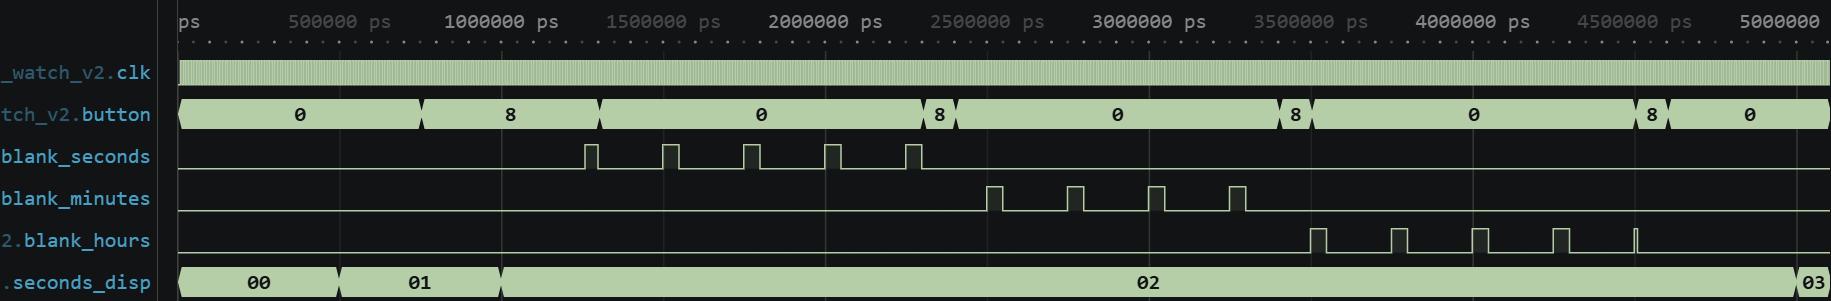
\includegraphics[width=\linewidth, height=0.1\textheight]{user_top_watch_v2_waveform}
		\caption{Measured waveform for user\_top\_watch\_v2.sv}
	\end{figure}
	
	The waveform displays inputs \textbf{clk}, and \textbf{button} and outputs \textbf{blank\_seconds}, \textbf{blank\_minutes}, \textbf{blank\_hours}, and \textbf{seconds\_disp}. We observe that:
	
	\begin{itemize}[noitemsep]
		\item \textbf{seconds\_disp} increments prior to long press of the button being registered.
		\item Initial pulse for \textbf{blank\_seconds} then 2Hz pulse before next button press.
		\item After next button press edit mode updated and \textbf{blank\_minutes} displays 2Hz pulse 
		\item After next button press edit mode updated and \textbf{blank\_hours} displays 2Hz pulse.
		\item After another button press we exit edit mode and \textbf{seconds\_disp} begins to increment again.
	\end{itemize}
	
	\subsection{User Top Watch V3}
	
	\begin{figure}[H]
		\centering
		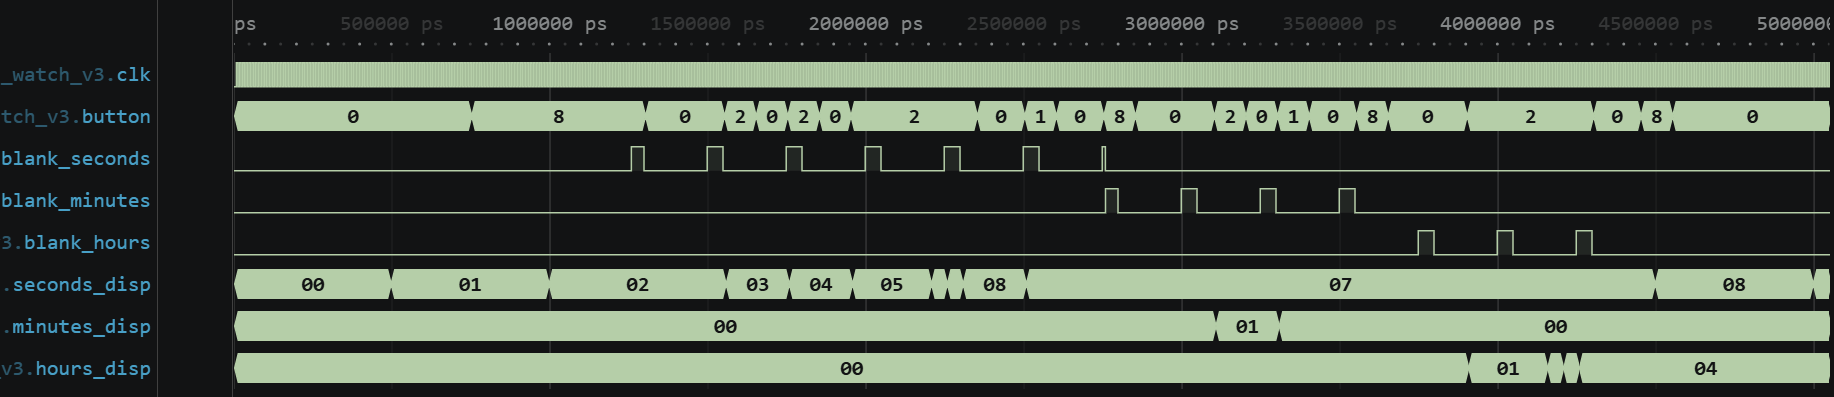
\includegraphics[width=\linewidth, height=0.15\textheight]{user_top_watch_v3_waveform}
		\caption{Measured waveform for user\_top\_watch\_v3.sv}
	\end{figure}
	
	The waveform displays inputs \textbf{clk}, \textbf{button}, and outputs \textbf{blank\_seconds}, \textbf{blank\_minutes}, \textbf{blank\_hours}, \textbf{seconds\_disp}, \textbf{minutes\_disp}, and \textbf{hours\_disp}. We observe that:
	
	\begin{itemize}[noitemsep]
		\item When in the seconds edit mode \textbf{seconds\_disp} increments each button press (2) and then auto increments once held for the appropriate cycle amount.
		\item \textbf{seconds\_disp} decrements when press (1) is asserted within edit mode.
		\item Button press (8) then enters minutes edit mode which increments \textbf{minutes\_disp} on button press (2) and decrements on button press (1). 
		\item Button press (8) then enters hours edit mode, again incrementing \textbf{hours\_disp} for each button press (2) or auto incrementing once held. 
	\end{itemize}
	
	\subsection{User Top Watch V4}
	\label{subsec:watchv4}
	
	\begin{figure}[H]
		\centering
		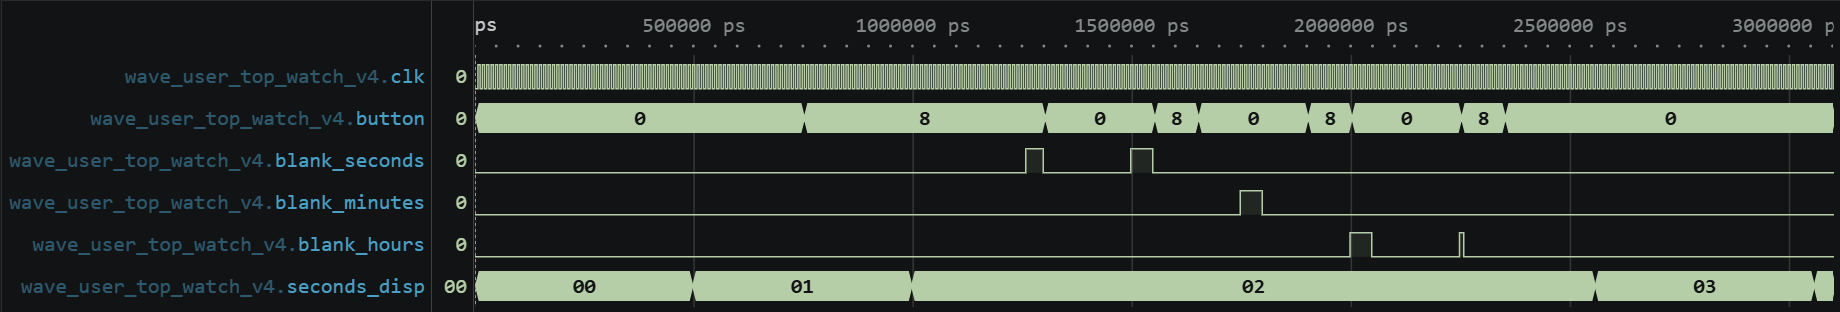
\includegraphics[width=\linewidth, height=0.15\textheight]{user_top_watch_v4_waveform}
		\caption{Measured waveform for user\_top\_watch\_v4.sv}
	\end{figure}
	
	The waveform displays inputs \textbf{clk}, \textbf{button}, and outputs \textbf{blank\_seconds}, \textbf{blank\_minutes}, \textbf{blank\_hours}, \textbf{seconds\_disp}. We observe that:
	
	\begin{itemize}[noitemsep]
		\item When transitioning from seconds edit mode to minutes edit mode our \textbf{second\_tick} resets so that the next tick upon exiting edit mode starts a second later. This is shown when \textbf{second\_disp} increments to 3 after exiting edit mode.
	\end{itemize}
	
	\section{Report 3}
	\begin{figure}[H]
		\centering
		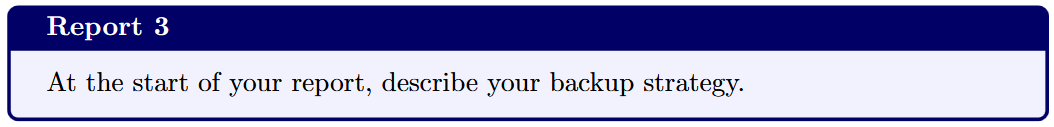
\includegraphics[width=\linewidth]{q_report3}
		\caption{Screenshot taken from Digital\_Watch\_Part\_1.pdf}
	\end{figure}
	
	 Repository fpga-digital-watch forked and modules completed locally. Changes are then committed and pushed to GitHub after a working session, or after a module has been implemented and tested.
	 
	 \section{Report 4}
	 \begin{figure}[H]
	 	\centering
	 	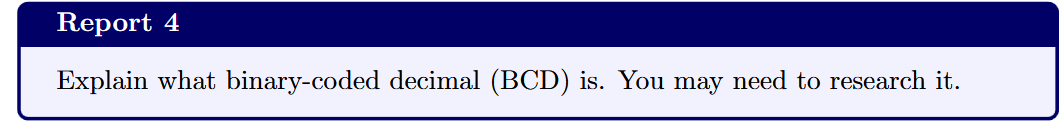
\includegraphics[width=\linewidth]{q_report4}
	 	\caption{Screenshot taken from Digital\_Watch\_Part\_1.pdf}
	 \end{figure}
	 
	 Binary-coded decimal (BCD) encodes a decimal number into a single binary digit for each place value.
	 
	 \section{Report 5}
	 \begin{figure}[H]
	 	\centering
	 	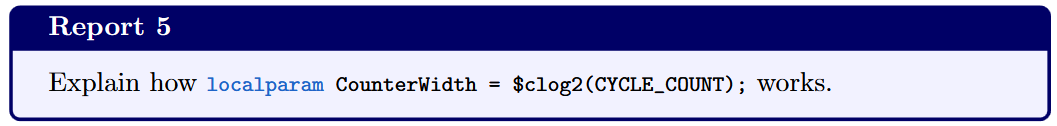
\includegraphics[width=\linewidth]{q_report5}
	 	\caption{Screenshot taken from Digital\_Watch\_Part\_1.pdf}
	 \end{figure}
	 
	 This allows us to set the minimum address width for CounterWidth according to the size of CYCLE\_COUNT without the need to state the bit width explicitly. \$2clog(CYCLE\_COUNT) will calculate the smallest power of 2 that will cover the memory required for CYCLE\_COUNT.
	 
	 \section{Report 6}
	 
	  \begin{figure}[H]
	 	\centering
	 	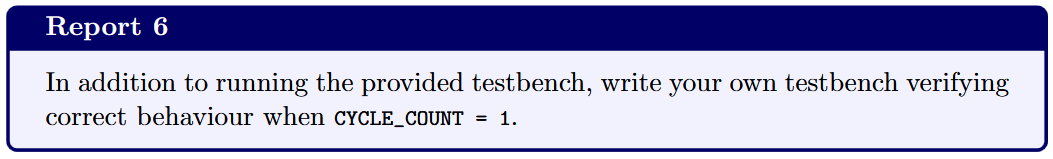
\includegraphics[width=\linewidth]{q_report6}
	 	\caption{Screenshot taken from Digital\_Watch\_Part\_1.pdf}
	 \end{figure}
	 
	 \begin{figure}[H]
	 	\centering
	 	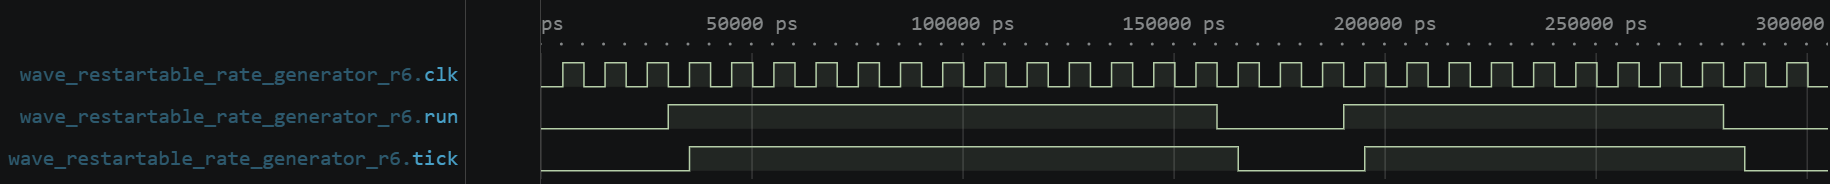
\includegraphics[width=\linewidth, height=0.1\textheight]{restartable_rate_generator_r6_waveform}
	 	\caption{Measured waveform for restartable\_rate\_generator.sv for case \textbf{CYCLE\_COUNT = 1}}
	 \end{figure}
	 
	 The waveform displays inputs \textbf{clk}, and \textbf{run}, and output \textbf{tick}. We observe that:
	 
	 \begin{itemize}[noitemsep]
	 	\item When \textbf{run} is low \textbf{tick} is low.
	 	\item \textbf{tick} follows \textbf{run} when high one cycle later. This one cycle delay is expected when implementing a Moore FSM.
	 \end{itemize}
	 
	 \section{Report 7}
	 
	 \begin{figure}[H]
	 	\centering
	 	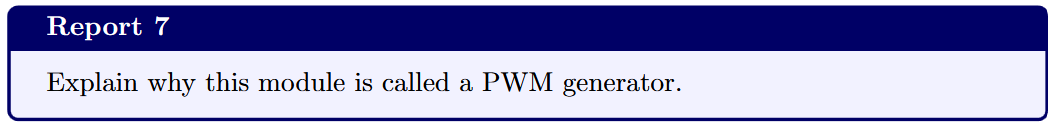
\includegraphics[width=\linewidth, height=0.07\textheight]{q_report7}
	 	\caption{Screenshot taken from Digital\_Watch\_Part\_1.pdf}
	 \end{figure}
	 
	 The module is called PWM generator as it generates a pulse wave and allows as to vary the pulse width with \textbf{DUTY\_CYLES}.
	 
	 \section{Report 8}
	 
	 \begin{figure}[H]
	 	\centering
	 	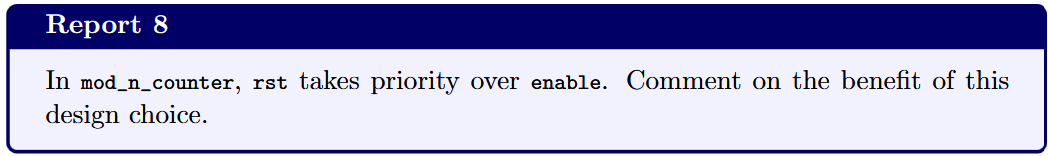
\includegraphics[width=\linewidth, height=0.1\textheight]{q_report8}
	 	\caption{Screenshot taken from Digital\_Watch\_Part\_1.pdf}
	 \end{figure}
	 
	 In our \textbf{mod\_n\_counter} module \textbf{rst} takes priority in the sequential logic within the flip-flop block so that the \textbf{count} is reset at the next rising clock edge. This ensures count is reset whilst keeping our circuit synchronous.
	 
	 \section{Report 9}
	 
	 \begin{figure}[H]
	 	\centering
	 	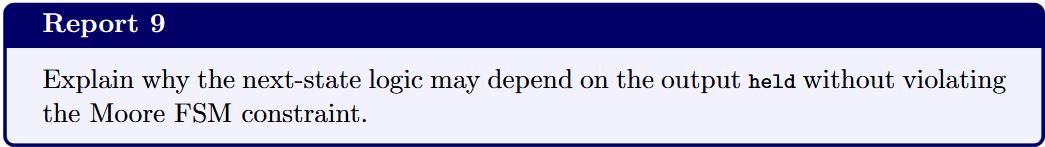
\includegraphics[width=\linewidth, height=0.09\textheight]{q_report9}
	 	\caption{Screenshot taken from Digital\_Watch\_Part\_1.pdf}
	 \end{figure}
	 
	 Our state has two variables \textbf{held} and \textbf{count} and there is no direct path to our output from our input. \textbf{held} is a registered output and therefore a part of our current state.
	 
	 \section{Report 10}
	 
	 \begin{figure}[H]
	 	\centering
	 	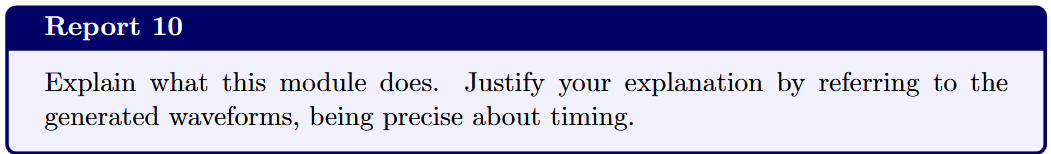
\includegraphics[width=\linewidth, height=0.1\textheight]{q_report10}
	 	\caption{Screenshot taken from Digital\_Watch\_Part\_1.pdf}
	 \end{figure}
	 
	Our \textbf{button\_hold\_pulse} module outputs a one clock cycle pulse once the button runs for the specified \textbf{HOLD\_CYCLES} within \textbf{button\_hold\_detect} module which has been instantiated in this module.
	
	\section{Report 11}
	
	\begin{figure}[H]
		\centering
		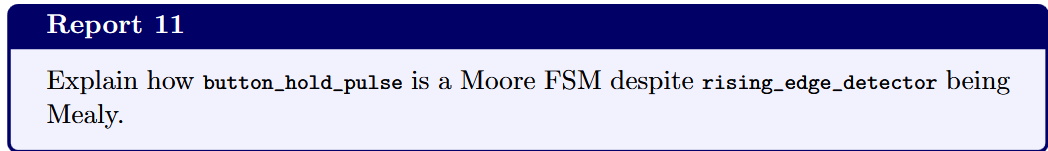
\includegraphics[width=\linewidth, height=0.1\textheight]{q_report11}
		\caption{Screenshot taken from Digital\_Watch\_Part\_1.pdf}
	\end{figure}
	
	The module \textbf{button\_hold\_pulse} is a Moore FSM as the input \textbf{held} is sent from \textbf{button\_hold\_detect} which is a Moore FSM. Meaning, the input to \textbf{button\_hold\_pulse} can only occur on a rising clock edge.
	
	\section{Report 12}
	
	\begin{figure}[H]
		\centering
		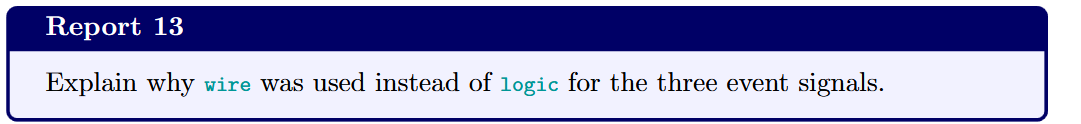
\includegraphics[width=\linewidth, height=0.1\textheight]{q_report12}
		\caption{Screenshot taken from Digital\_Watch\_Part\_1.pdf}
	\end{figure}
	
		\begin{figure}[H]
		\centering
		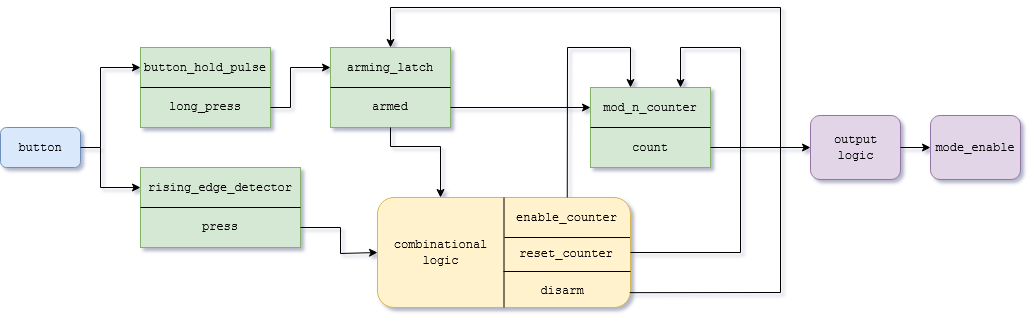
\includegraphics[width=\linewidth, height=0.2\textheight]{q_report12_block_diagram}
		\caption{Block diagram created using draw.io}
	\end{figure}
	
	The following combinational logic was used to drive our \textbf{mod\_n\_counter}:
	
	\begin{itemize}[noitemsep]
		\item \textbf{enable\_counter} is assigned \textbf{press \&\& armed} which ensures our \textbf{arming\_latch} has been armed before registering a button press to enable our counter.
		\item \textbf{reset\_counter} is simply assigned to \textbf{disarm}.
		\item \textbf{disarm} is assigned \textbf{press \&\& armed \&\& (count == 2)} to disarm our latch and reset our counter on the press that steps past the last mode. This ensures the circuit registers a new long press before re-entering edit mode.
	\end{itemize}
	
	\section{Report 13}
	
	\begin{figure}[H]
		\centering
		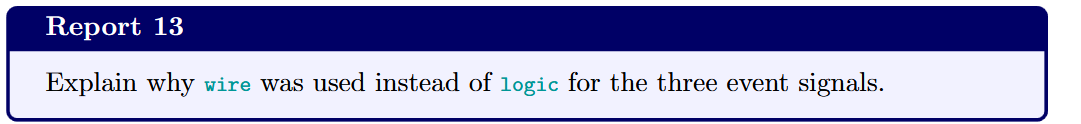
\includegraphics[width=\linewidth, height=0.08\textheight]{q_report13}
		\caption{Screenshot taken from Digital\_Watch\_Part\_1.pdf}
	\end{figure}
	
	We can use wire since we are using combinational signals driven by continuous assignments and do not need to store a value.
	
	\section{Report 14}
	
	\begin{figure}[H]
		\centering
		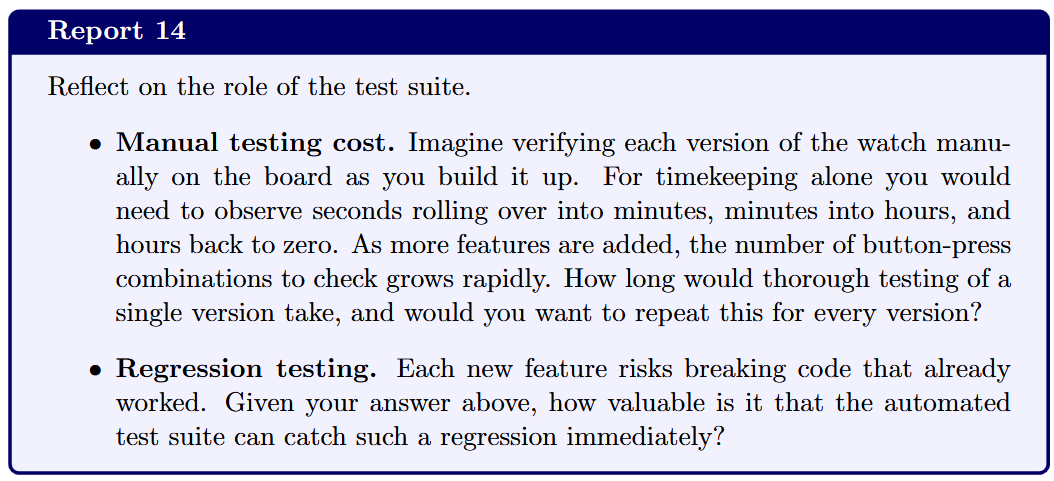
\includegraphics[width=\linewidth, height=0.3\textheight]{q_report14_p1}
		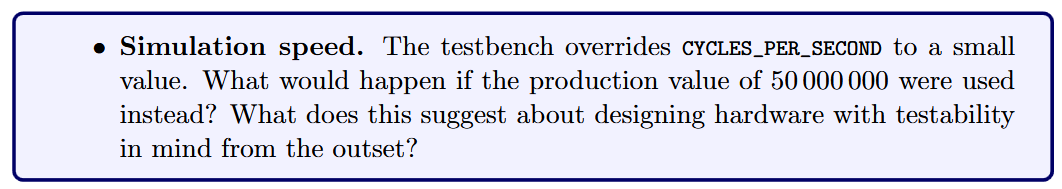
\includegraphics[width=\linewidth, height=0.12\textheight]{q_report14_p2}
		\caption{Screenshot taken from Digital\_Watch\_Part\_1.pdf}
	\end{figure}
	
	To thoroughly test our stop watch manually we would need to observe that each tick increments correctly which would take 24 hours at least. This is without factoring in the button presses which increases the testing time required and complexity of the testing exponentially with each input added to the system. Every new version would need to be tested the same amount of time at least, although likely longer.
	\\
	\\
	\noindent Regression testing ensures that previous test cycles are not wasted and that we are safely building upon our already implemented code. Given that significant amounts of time may have already gone into testing previous versions we want to be able to pinpoint if any new additions break our existing code where possible
	\\
	\\
	\noindent Setting the production values to 50,000,000 would make it difficult to verify within our testing environment and especially if we were manually test our design. These speeds exceed human perception making verification impossible depending on which module we test. Designing hardware with testability from the outset makes sure we can use values that are easier to follow and verify which can then be scaled during production
	
	\section{Report 15}
	
	\begin{figure}[H]
		\centering
		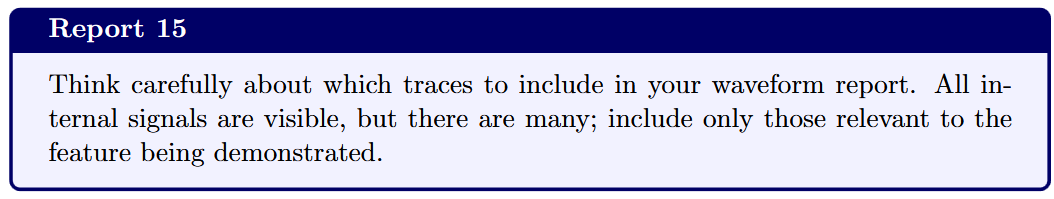
\includegraphics[width=\linewidth, height=0.12\textheight]{q_report15}
		\caption{Screenshot taken from Digital\_Watch\_Part\_1.pdf}
	\end{figure}
	
	See \autoref{subsec:watchv4}.
	
	\section{Report 16}
	
	\begin{figure}[H]
		\centering
		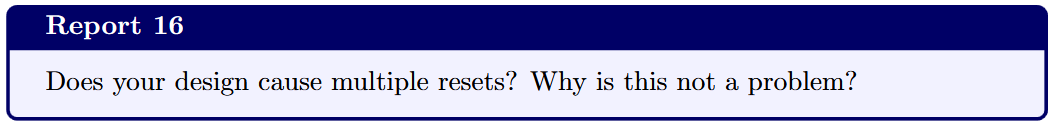
\includegraphics[width=\linewidth, height=0.09\textheight]{q_report16}
		\caption{Screenshot taken from Digital\_Watch\_Part\_1.pdf}
	\end{figure}
	
	This will cause multiple resets as the button is not using a rising edge detector, so we may register a brief press for multiple rising clock edges. This will not cause issues as the \textbf{run} will assert high when transitioning to the next \textbf{edit\_mode}.
	
	\section{Report 17}
	
	\begin{figure}[H]
		\centering
		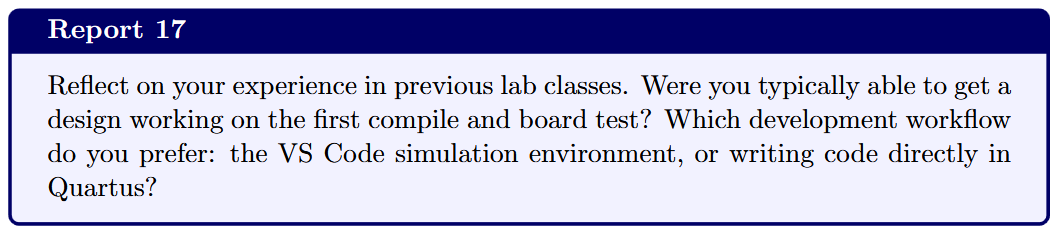
\includegraphics[width=\linewidth, height=0.14\textheight]{q_report17}
		\caption{Screenshot taken from Digital\_Watch\_Part\_1.pdf}
	\end{figure}
	
	Most designs did not work correctly the first time implemented on the board or there produced unintended display issues. \\
	\\
	\noindent I prefer working in the simulation environment. It is less time consuming and the asserts give feedback as to the exact issues with our module which improves debugging. Although you miss the physical feedback of the FPGA, it is satisfying to run your code directly and have this work after verification which saves a lot of compilation time compared to Quartus.
	
	\section{Report 18}
	
	\begin{figure}[H]
		\centering
		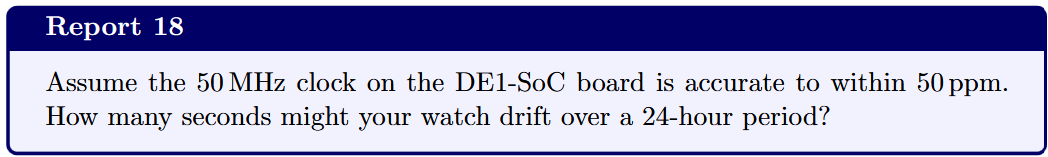
\includegraphics[width=\linewidth, height=0.1\textheight]{q_report18}
		\caption{Screenshot taken from Digital\_Watch\_Part\_1.pdf}
	\end{figure}
	
	Assuming 50MHz clock we will have between 50,002,500Hz and 49997500Hz drift. Assuming maximum drift for a 24-hour period we will get 1.00005 x 86,400 seconds = 86,404.32. So we will get approximately 4.32 seconds of drift every 24 hours.
		
\end{document}